% ****** Start of file apssamp.tex ******
%
%   This file is part of the APS files in the REVTeX 4 distribution.
%   Version 4.0 of REVTeX, August 2001
%
%   Copyright (c) 2001 The American Physical Society.
%
%   See the REVTeX 4 README file for restrictions and more information.
%
% TeX'ing this file requires that you have AMS-LaTeX 2.0 installed
% as well as the rest of the prerequisites for REVTeX 4.0
%
% See the REVTeX 4 README file
% It also requires running BibTeX. The commands are as follows:
%
%  1)  latex apssamp.tex
%  2)  bibtex apssampya
%  3)  latex apssamp.tex
%  4)  latex apssamp.tex
%
\documentclass[pra,groupedaddress,amsmath,amssymb, column]{revtex4}

\setlength{\parindent}{10mm}
%\documentclass[twocolumn,pra,groupedaddress,amsmath,amssymb]{revtex4}
%\documentclass[twocolumn,pra,showpacs,groupedaddress,superscriptaddress,amsmath,amssymb]{revtex4}
%\documentclass[preprint,showpacs,preprintnumbers,amsmath,amssymb]{revtex4}

% Some other (several out of many) possibilities
%\documentclass[preprint,aps]{revtex4}
%\documentclass[preprint,aps,draft]{revtex4}
%\documentclass[pra]{revtex4}% Physical Review B

\usepackage{graphicx}% Include figure files
\usepackage{braket}
\usepackage{amsmath}
\usepackage{bm}% bold math
\usepackage{subfigure} 
%\usepackage{dcolumn}% Align table columns on decimal point


\begin{document}

\title{Stats 315a: Statistical Learning \\ Problem Set 1}
\author{Dong-Bang Tsai}
    \email{dbtsai@stanford.edu}
\affiliation{Department of Applied Physics, Stanford University, Stanford, California 94305, USA}



\date{\today}
\maketitle


\section*{Problem 1}
\subsection*{(a)}
MATLAB is used for this homework instead of R; I already asked professor if we can use MATLAB, and he said it's okay. My teammates are Jin Chen, and Wenqiong Guo. Basically, the code will generate a training sample of size 100 for each class, as well as a test sample of 5,000 per class. Then, we use linear regression and K-nearest neighbour (trained with training sample) to do the classification on test sample.
\begin{verbatim}
\end{verbatim}

\section*{Problem 2 (ESL 2.4)}
The squared distance from any sample point to the origin has a $\chi_p^2$ distribution with mean $p$; therefore, since a prediction point $x_0$ is drawn from this distribution, it will have a expected squared distance $p$ from the origin. 

Because $z_i=a^Tx_i$, and $a$ is independent from $x_i$, we can conclude that $z_i \sim N$, normal distribution. Now, let's calculate the expectation value of $z_i$. We know that for a $p$ dimensional vector $a$ 
\begin{align}
E(z) = E(a^Tx) = a^TE(x) = 0
\end{align}

The co-variant can be given by
\begin{align}
Cov(a^Tx) = a^Ta = 1
\end{align}
As a result, we get $z_i \sim N(0,1)$, and the expected squared distance will be $E(z^2) = 1$.



\section*{Problem 3 (ESL 2.7)}
\subsection*{(a)}
For linear regression, the exact solution can be given by
\begin{align}
\hat{\beta} = (\mathbf{X}^T\mathbf{X})^{-1}\mathbf{X}^T\mathbf{y}
\end{align}
therefore, the predicted value for a given input will be
\begin{align}
\hat{f}(x_0) = x_0^T\hat{\beta}
\end{align}
Compare with the desired form of the estimator,
\begin{align}
\hat{f}(x_0) =\sum_{i=1}^{N}l_i(x_0; \mathbf{X})y_i \label{3a}
\end{align}
it's found that
\begin{align}
l_i(x_0; \mathbf{X}) = x_0^T(\mathbf{X}^T\mathbf{X})^{-1}x_i^T
\end{align}
Therefore, linear regression is the member of this class of estimators. 

For k-nearest-neighbour regression, the estimator is 
\begin{align}
\hat{f}(x_0) = \frac{1}{k}\sum_{x_i\in N_k(x_0)}y_i
\end{align}
where $N_k(x_0)$ is the neighbourhood of $x_0$ defined by the $k$ closest points $x_i$ in the training sample. Now, compare with the desired estimator form, it's found that
\begin{align}
l_i(x_0; \mathbf{X}) =\left\{ 
\begin{array}{l}
0\;\;\;\;\text{$x_i \not\in N_k(x_0)$} \\
\frac{1}{k}\;\;\;\text{$x_i\in N_k(x_0)$}
 \end{array}\right.
\end{align}
Therefore,  k-nearest-neighbour regression is the member of this class of estimators. 

\subsection*{(b)}
Using Eq.~(2.25) in the textbook, the conditional mean squared error can be rewritten as
\begin{align}
E_{\mathbf{y|x}}(f(x_0) - \hat{f}(x_0))^2&= E_{\mathbf{y|x}}(\hat{f}(x_0) - E_{\mathbf{y|x}}\hat{f}(x_0))^2 + (E_{\mathbf{y|x}}\hat{f}(x_0) - {f}(x_0))^2 \nonumber\\
&=Var_{\mathbf{y|x}}(\hat{f}(x_0)) + Bias^2_{\mathbf{y|x}}(\hat{f}(x_0)) \label{3b}
\end{align}
Substitute Eq.~(\ref{3a}) into Eq.~(\ref{3b}), we have
\begin{align}
Var_{\mathbf{y|x}}(\hat{f}(x_0))  &= Var_{\mathbf{y|x}}\left(\sum_{i=1}^{N}l_i(x_0; \mathbf{X})y_i\right)  \nonumber\\
&=\sum_{i=1}^{N}l_i(x_0; \mathbf{X})Var_{\mathbf{y|x}}\left(y_i\right) \nonumber\\
&=\sum_{i=1}^{N}l_i(x_0; \mathbf{X})\sigma^2
\end{align}
and
\begin{align}
Bias_{\mathbf{y|x}}(\hat{f}(x_0)) &= Bias_{\mathbf{y|x}}\left(\sum_{i=1}^{N}l_i(x_0; \mathbf{X})y_i\right)  \nonumber\\
&= E_{\mathbf{y|x}}\sum_{i=1}^{N}l_i(x_0; \mathbf{X})y_i- {f}(x_0)\nonumber\\
&= \sum_{i=1}^{N}l_i(x_0; \mathbf{X})f(x_i)- {f}(x_0)
\end{align}

\subsection*{(c)}

For the unconditional mean squared error, we have
\begin{align}
E_{\mathbf{y,x}}(f(x_0) - \hat{f}(x_0))^2&=Var_{\mathbf{y,x}}(\hat{f}(x_0)) + Bias^2_{\mathbf{y,x}}(\hat{f}(x_0)) 
\end{align}
Therefore, the variance will be
\begin{align}
Var_{\mathbf{y,x}}(\hat{f}(x_0))  &=  E_{\mathbf{y,x}}(\hat{f}(x_0) - E_{\mathbf{y,x}}\hat{f}(x_0))^2\nonumber \\
&= E_xE_{\mathbf{y|x}}(\hat{f}(x_0) - E_xE_{\mathbf{y|x}}\hat{f}(x_0))^2\nonumber\\
&= E_xE_{\mathbf{y|x}}\left(\sum_{i=1}^{N}l_i(x_0; \mathbf{X})y_i- E_x\left(\sum_{i=1}^{N}l_i(x_0; \mathbf{X})f(x_i) \right)\right)^2\nonumber\\
&=E_x\left[ E_{\mathbf{y|x}}\left(\sum_{i=1}^{N}l_i(x_0; \mathbf{X})y_i\right)^2- 2E_{\mathbf{y|x}}\left(\sum_{i=1}^{N}l_i(x_0; \mathbf{X})y_i\right) \left(\sum_{i=1}^{N}l_i(x_0; \mathbf{X})f(x_i) \right)\right. \nonumber\\
 &\;\;\; \left.+E_x\left(\sum_{i=1}^{N}l_i(x_0; \mathbf{X})f(x_i) \right)\left(\sum_{i=1}^{N}l_i(x_0; \mathbf{X})f(x_i) \right) \right]\nonumber\\
&= E_xE_{y|x}\left(  \sum_{i=1}^{N}l_i(x_0; \mathbf{X})y_i - \sum_{i=1}^{N}l_i(x_0; \mathbf{X})f(x_i) \right)^2  + E_x\left(E_x(\sum_{i=1}^{N}l_i(x_0; \mathbf{X})f(x_i)) -\sum_{i=1}^{N}l_i(x_0; \mathbf{X})f(x_i)  \right)^2\nonumber\\
&= E_xVar_{y|x}(\hat{f}(x_0))  + Var_x\left(\sum_{i=1}^{N}l_i(x_0; \mathbf{X})f(x_i) \right) \nonumber\\
&= E_x\left(\sum_{i=1}^{N}l_i(x_0; \mathbf{X})\sigma^2\right)+Var_x\left(\sum_{i=1}^{N}l_i(x_0; \mathbf{X})f(x_i) \right)
\end{align}
The Bias will be
\begin{align}
Bias_{y,x}(\hat{f}(x_0) &=  E_{\mathbf{y,x}}\hat{f}(x_0) - E_x{f}(x_0)\nonumber\\
&= E_x( E_{y|x}\hat{f}(x_0) - f(x_0))  \nonumber\\
&= E_x(  \sum_{i=1}^{N}l_i(x_0; \mathbf{X})f(x_i) - f(x_0)  ) \nonumber\\
&=E_{x}Bias_{y|x}(\hat{f}(x_0) )
\end{align}

\subsection*{(d)}
Compare the result in (b), and (c), we find that the unconditional squared bias is the expected value respected to $X$ of conditional squared bias. $E_{x}Bias_{y|x}(\hat{f}(x_0) )= Bias_{x,y}(\hat{f}(x_0))$

The unconditional variance will be the expected value respected to $X$ of conditional variance with extra variance term.
\begin{align}
Var_{y,x}(\hat{f}(x_0)) = E_xVar_{y|x}(\hat{f}(x_0))+Var_x\left(\sum_{i=1}^{N}l_i(x_0; \mathbf{X})f(x_i) \right)\nonumber
\end{align}



\section*{Problem 4}
\subsection*{(a)}
Let $\hat{\beta}$ be the least squares estimation over a set of training data $(x_1,y_1),...,(x_n,y_n)$ using
\begin{align}
R_{tr}(\hat{\beta}) = \frac{1}{N}\sum_{1}^N(y_i - \hat{\beta}^Tx_i)^2
\end{align}, while $\tilde{\beta}$ is the least squares estimation over another set of training data $(\tilde{x}_1,\tilde{y}_1),...,(\tilde{x}_n,\tilde{y}_n)$ drawn at random from the same population as the first training data using
\begin{align}
R_{te}(\tilde{\beta}) = \frac{1}{M}\sum_{1}^M(\tilde{y}_i - \tilde{\beta}^T\tilde{x}_i)^2
\end{align}

Since both training data are drawn from the same population, if they are randomly  picked up, we can say
\begin{align}
E[R_{tr}(\hat{\beta})] = E[R_{te}(\tilde{\beta}) ]\label{4equal}
\end{align}, which can be formally proven by
\begin{align}
E[R_{tr}(\hat{\beta})] &= E[ \frac{1}{N}\sum_{1}^N({y}_i - \hat{\beta}^T{x}_i)^2 ]\nonumber\\
&= \frac{1}{N}E[\sum_{1}^N({y}_i - \hat{\beta}^T{x}_i)^2 ]\nonumber\\
&=  \frac{1}{M}E[\sum_{1}^M({y}_i - \hat{\beta}^T{x}_i)^2 ]\nonumber\\
&=  \frac{1}{M}E[\sum_{1}^M(\tilde{y}_i - \tilde{\beta}^T\tilde{x}_i)^2 ]\nonumber\\
&=E[R_{te}(\tilde{\beta}) ]
\end{align}

Also, $\tilde{\beta}$ is the least squares estimation over $(\tilde{x}_1,\tilde{y}_1),...,(\tilde{x}_n,\tilde{y}_n)$, so
\begin{align}
 \frac{1}{M}\sum_{1}^M(\tilde{y}_i - \tilde{\beta}^T\tilde{x}_i)^2 &\leq  \frac{1}{M}\sum_{1}^M(\tilde{y}_i - \hat{\beta}^T\tilde{x}_i)^2\nonumber\\
  \Rightarrow R_{te}({\tilde{\beta}})&\leq R_{te}({\hat{\beta}})\nonumber\\
 \therefore E[R_{te}({\tilde{\beta}})]&\leq E[R_{te}({\hat{\beta}})]\label{4inequal}
 \end{align}
With Eq.~(\ref{4equal}) and Eq.~(\ref{4inequal}), we get
\begin{align}
  \therefore E[R_{tr}({\hat{\beta}})]&\leq E[R_{te}({\hat{\beta}})]\label{4inequal}
 \end{align}

\section*{Problem 5 (ESL 3.2)}
\subsection*{Method 1}
For each point $x_0$, forming a $95\%$ confidence interval implies that we need to know the confidence interval for $\hat{\beta}$, and using linear function $a^T\hat{\beta}$ to construct the $95\%$ confidence band. Since $\hat{\beta}\sim N(\beta, (\mathbf{X}^T\mathbf{X})^{-1}\sigma^2))$, we can obtain the $1-2\alpha$ confidence interval for $\beta$ as
\begin{align}
\left( \hat{\beta} - z^{(1-\alpha)}\sqrt{(\mathbf{X}^T\mathbf{X})^{-1}}{\sigma},  \hat{\beta} + z^{(1-\alpha)}\sqrt{(\mathbf{X}^T\mathbf{X})^{-1}}{\sigma}\right)
\end{align}
where $z^{(1-\alpha)}$ is the $1-\alpha$ percentile of the normal distribution. (Note that if we replace the $\alpha$ to known value $\hat{\alpha}$, the distribution will become $t$ distribution, and it normally become negligible as the sample increases; therefore, we typically use the normal quartiles.)
As a result, the confidence interval from each input point $x_0$ will be
\begin{align}
\left( a^T\hat{\beta} - z^{(1-\alpha)}\sqrt{a^T(\mathbf{X}^T\mathbf{X})^{-1}a}{\sigma},  \hat{\beta} + z^{(1-\alpha)}\sqrt{a^T(\mathbf{X}^T\mathbf{X})^{-1}a}{\sigma}\right)
\end{align}
where $y_0 = a^T\hat{\beta} = \sum_{j=0}^3\hat{\beta}_jx_0^j$. For $95\%$, $\alpha$ is $0.025$.

\subsection*{Method 2}
From Eq.~(3.15) from textbook, the confidence set for $\beta$ can be given by
\begin{align}
C_\beta = \left\{\beta|(\hat{\beta}-\beta)^T\mathbf{X}^T\mathbf{X}(\hat{\beta}-\beta)\le {\sigma}^2{\chi^2_4}^{(1-2\alpha)}\right\}
\end{align}
Therefore, the $95\%$confidence band from each input point $x_0$ will be
\begin{align}
\left( a^T\hat{\beta} -\sqrt{a^T(\mathbf{X}^T\mathbf{X})^{-1}a{\chi^2_4}^{(1-2\alpha)}}{\sigma},  \hat{\beta} + \sqrt{a^T(\mathbf{X}^T\mathbf{X})^{-1}a{\chi^2_4}^{(1-2\alpha)}}{\sigma}\right)
\end{align}
where  $\alpha$ is $0.025$, and ${\chi_l^2}^{(1-\alpha)}$ is the chi-squared distribution on $l$ degrees of freedom. (Similar to the discussion in method 1, if we don't know the $\alpha$, but we know $\hat{\alpha}$ which can be calculated from training set, the chi-squared distribution will be replaced by $F_{p_1-p_0,M-p_1-1}$ distribution.)

According to simulation result shown in the figure,  it's observed that Method 2 has wider confidence band. 
\begin{figure}
	\begin{center}
		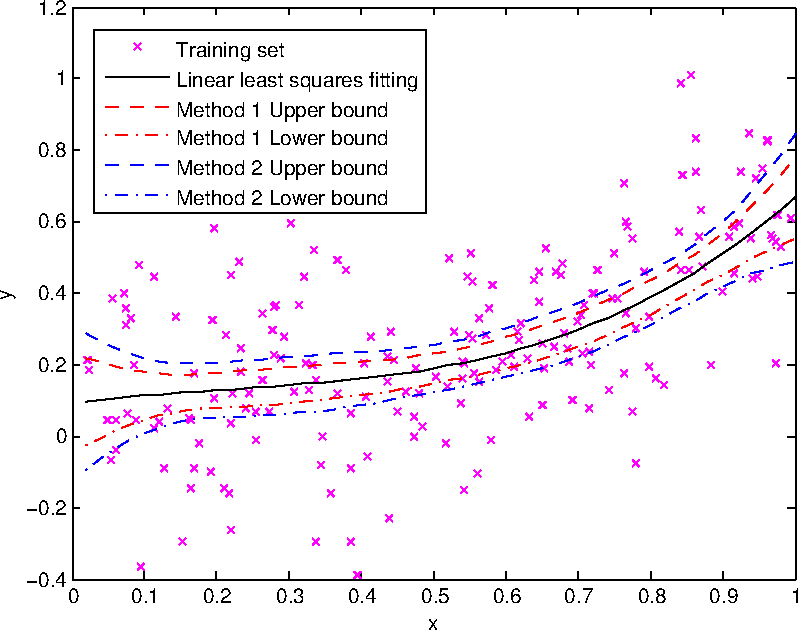
\includegraphics[width=1.\textwidth]{Q5.pdf} 
	\end{center}
\end{figure}


\begin{verbatim}
% HW1, Q5 (ESL3.2)
% Dong-Bang Tsai
clear all;

N = 200;            % N of training set
alpha = (1-0.95)/2; % 95% confidence interval
sigma = 0.2;        % Gaussian random noise

% The training set
beta = randn(4,1);
x_points = rand(N,1); 
X = [ones(N,1),x_points,x_points.^2,x_points.^3]; 
y = X*beta + normrnd(0,sigma,N,1);
% Learned hypothesis
hat_beta = ((X'*X))\X'*y; 

% Plot array
N_plot = 50;
x_plot_points = [1/N_plot:1/N_plot:1]';
a = [ones(N_plot,1),x_plot_points,x_plot_points.^2,x_plot_points.^3];

% Compute the confidence band
hat_sigma = sqrt( 1/(N-4)*sum( (X*beta-y).^2 ) );
delta1 = norminv(1-alpha)*sqrt(diag(a*((X'*X)\a')))*hat_sigma;
delta2 = sqrt(diag(a*((X'*X)\a'))*chi2inv(1-2*alpha,4))*hat_sigma;

plot(x_points,y(:,1),'mx'); 
hold on;
plot(x_plot_points,a*beta,'k-');
plot(x_plot_points,a*beta + delta1,'r--'); 
plot(x_plot_points,a*beta - delta1,'r-.');
plot(x_plot_points,a*beta + delta2,'b--'); 
plot(x_plot_points,a*beta - delta2,'b-.');
xlabel('x'); ylabel('y');
legend('Training set','Linear least squares fitting','Method 1 Upper bound', 'Method 1 Lower bound', 'Method 2 Upper bound', 'Method 2 Lower bound');
hold off;
\end{verbatim}


\section*{Problem 6}
\subsection*{(a)}
When $p \gg N$, the columns of $X$ are not lineraly independent which implies $X$ isn't of full rank. Therefore, the solution of least squares given by $\hat{\beta}=(X^TX )^{-1}X^T y$ will not be uniquely defined since $X^TX$ is singular, and the residuals of the solution will be $0$. The solution is unique only if $X$ has a full column rank, and $X^TX$ is positive definite. 


\subsection*{(b)}
In the ridge regression approach, the equation we are trying to solve is 
\begin{align}
(X^TX +  \lambda I)\beta = X^T y
\end{align}
The solution can be given by $\hat{\beta}_{\lambda}=(X^TX +  \lambda I)^{-1}X^T y$.  We add positive constant to diagonal of $X^TX$; therefore, $(X^TX +  \lambda I)^{-1}$ is non-singular, even if $X^TX$ is not of full rank. As a result, the solution always exists, and is unique.
\subsection*{(c)}
As we show that the solution of ridge regression is $\hat{\beta}_{\lambda}=(X^TX +  \lambda I)^{-1}X^T y$, if we try to get the $\lambda$ smaller, it will eventually become least squares solution which is $\hat{\beta}_{\lambda}=(X^TX )^{-1}X^T y$.
\subsection*{(d)}
Using $X=UDV^T$
\begin{align}
\hat{\beta}_{\lambda}&=(X^TX +  \lambda I)^{-1}X^T y \nonumber\\
				       &=\left( VD^TU^TUDV^T  + \lambda I \right)VDU^T y \nonumber\\
                                      &=V\left(D^2 + \lambda I \right)V^TDU^T y \nonumber\\
                                      &=V\left(D^2 + \lambda I \right)DU^T y
\end{align}
\end{document}

